\setchapterpreamble[u]{\margintoc}

\chapter{Droplet Generation in Corrugated Ligaments}
\labch{breakup}

% Rearrangement of liquid volumes in ligaments
Ligaments constitute the penultimate stage in the complex sequence 
of capillary-driven topological changes that are 
typical of liquid fragmentation processes, 
finally resulting in the generation of polydisperse collections of drops. 
In the context of the present body of work, we shall 
only concern ourselves with the dynamics of Newtonian ligaments, 
which are well described by the Navier-Stokes equations 
at the incompressible and isothermal limits. 
The rearrangement of the liquid volumes that constitute
the ligaments play a key role in determining the size 
of the droplets that emerge immediately after the disintegration
of the thread-like structure (Fig. \ref{lig_stretch} ).  

\begin{marginfigure}[3cm]
\centering
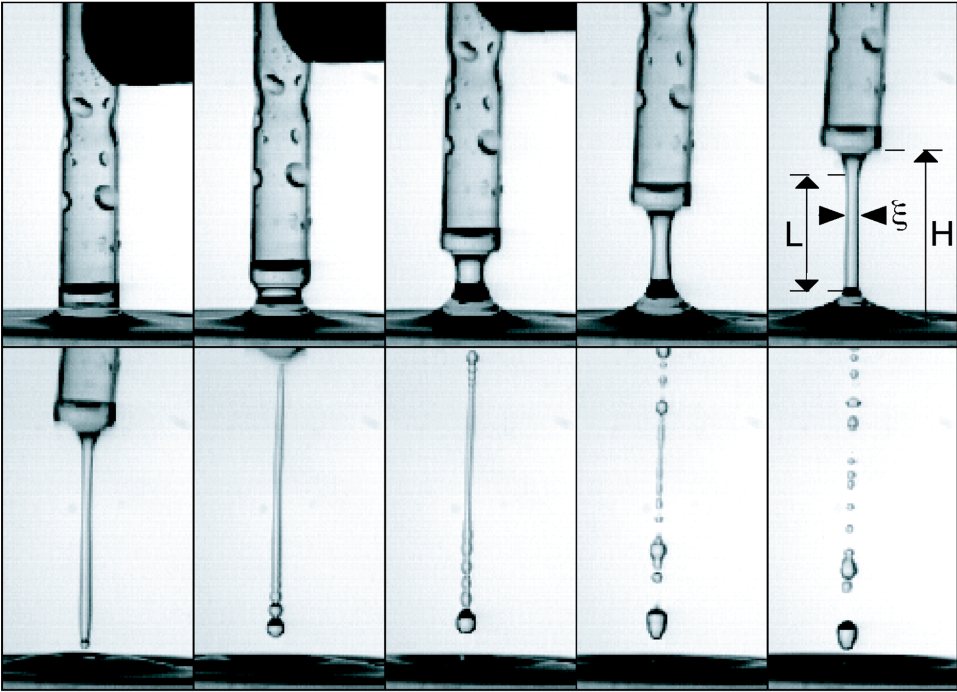
\includegraphics{plots/ligament_breakup/lig_mar_vill_pof04.png}
\caption{Fragmentation of stretched liquid (Newtonian) ligaments formed 
	immediately after retraction of a capillary tube. 
	Image reproduced from Marmottant \& Villermaux \cite{vill_3}.
       	The complex rearrangement of the liquid volumes 
	inside the ligament plays a key role in its subsequent 
	disintegration into droplet of various sizes. 
	}
\label{lig_stretch}
\end{marginfigure}

The dynamics of these rearrangements prior to breakup are 
governed by non-linear interactions between several 
physical mechanisms such as the growth and propagation of capillary 
waves along the ligament surface, remnants of the internal flow, 
stretching induced either by the surrounding gas flow or by 
acceleration of the liquid into the surrounding medium itself,
not to mention the dissipative effects of viscosity.  
Although we present a convoluted picture of ligament dynamics prior
to breakup, it is ultimately the capillary force that drives the 
eventual topology change from the thread-like structure to that of the drop. 
The primary role of the both the inertial and viscous forces is to oppose 
or dampen the destabilizing effects of the capillarity induced deformations.   
An additional mechanism to consider is the merger or coalescence of the 
newly created droplets (post-breakup) along the axis of the former ligament
structure, or with droplets originating from other sources in the near vicinity. 
The generation of drops whose diameters are significantly larger than the 
width of original ligament are predominantly driven by the aforementioned coalescences.  
Therefore, considering the combined effects of the above mechanisms, we expect a significant
departure of the resulting drop size distribution from that predicted by the  
classical analysis of the Rayleigh-Plateau instability \cite{rayleigh1879a,rayleigh1879b}. 


% Corrugation-coalescence model
Linear theory based on the the Rayleigh breakup of infinitely
long liquid cylinders in a quiescent medium predicts the disintegration
of the thread along regular intervals, the length of which is governed
by the fastest growing spatial frequency. 
The drops generated according to this model would be uniform in
size, in sharp contrast to the significant variances in the size distributions
observed in reality.  
Even in the simpler case of decaying liquid jets, 
non-linearities near the breakup zone kick into effect beyond
the initial exponential growth phase predicted by linear theory, 
eventually resulting in the jet breaking up into 
``main'' drops and significantly smaller ``satellite'' droplets 
\sidenote{Refer to the high quality photographs in 
the work of Rutland and Jameson \cite{rutland1971non}, where they demonstrate 
the formation of ``satellite'' droplets that manifest due to the non-linear effects
driving the jet breakup.}. 
Thus, simply taking into account the non-linear effects driving the breakup would
lead to a bimodal distribution of droplet size, but this explanation 
still fails to account for the broad distribution of sizes observed in 
the outcomes of the majority of natural \cite{nature} and industrial \cite{industrial} processes. 


As we have seen in the previous chapter, there are several hypotheses 
in existing literature \sidecite{vill_1} 
that attempt to model the underlying physical mechanisms 
that are responsible for the selection of droplet size. 
A model first proposed by Villermaux and coworkers \sidecite{vill_2,vill_4}
asserts that the variance in the droplet sizes is strongly 
correlated to the initially corrugated shape of the 
ligament, from which the drops originate. 
In this model, the corrugated ligament is represented as a collection 
of `blobs' (see Fig. \ref{blobs}), with the continuous interaction between 
such blobs throughout the destabilization phase accounting for the 
rearrangement and concomitant aggregation of the liquid volumes prior to breakup. 
\marginnote{
The corrugation-coalescence mechanisn has been 
popularized in several studies such as \cite{vill_3,vill_1,vill_5,vill_6,vill_7},
and more recently in \cite{bonn,mckinley}.
}
The key parameter concerning the predictions of this model 
is $n$, which characterizes the corrugations in the initial 
geometrical shape of the ligament, defined as  

\begin{align}
	n \equiv \frac{1}{\left(\langle d^{2} \rangle - \langle d \rangle^{2} \right) / \langle d \rangle^{2}} \, ,  
\end{align}

\begin{marginfigure}
\centering
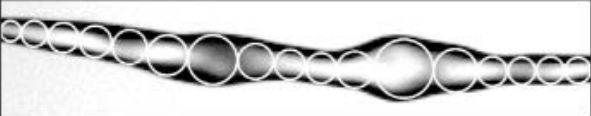
\includegraphics{plots/ligament_breakup/lig_protoblobs.png}
\caption{Representation of the liquid volumes in an isolated ligament as `blobs'
	of sizes $d$ matching the corresponding the local thicknesses, 
	just before the destabilization into droplets. 
	Image reproduced from Villermaux \cite{vill_1}.
	}
\label{blobs}
\end{marginfigure}


where the quantities in the brackets $\langle \quad \rangle$ represent the mean
and the diameters $d_i$ correspond to that of the blobs as shown in Fig. \ref{blobs}.
These studies essentially demonstrate that the degree of polydispersity 
in the drop sizes can be simply explained by examining the 
degree of ``smoothness'' in the initial geometry of the ligaments, 
with the standard deviation or distribution width of the size of the 
emerging drops scaling as $1 / \sqrt{n}$. 
As a corollary to this prediction, a broader distribution of drop sizes arise out
of the disintegration of strongly corrugated (rough) ligaments, whereas smoother 
ligaments with uniform thickness lead to a narrower (monodisperse) distributions. 


\begin{marginfigure}
\centering
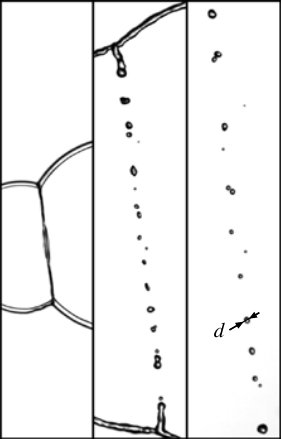
\includegraphics{plots/ligament_breakup/lig_sheet_hole.png}
\caption{Successive stages in the breakup of a ligament into drops. 
	The system shown here is that of a perforated liquid sheet, 
	where the growth of such perforations due to capillary retraction 
	of the liquid rims lead to the formation of networks of connected ligaments. 
	Image reproduced from Lhuissier and Villermaux \cite{sheet_hole}.
	}
\label{lig_network}
\end{marginfigure}


% Difficulties associated 
Over the last two decades, a handful of studies have been conducted 
with the aim of carrying out detailed observations surrounding 
the aforementioned ``coalescence cascade'', whereby the drops 
constitutive of the ligament tend to coalesce and form larger drops
as and when they detach from the initial thread-like structure.
Most notable amongst those studies is the one by Marmottant and Villermaux \cite{vill_3},
wherein they illustrate the successive stages of the disintegration of 
liquid ligaments formed when capillary tubes are rapidly retracted from 
the surface of a liquid pool (refer to Fig. \ref{lig_stretch}). 
Another set of observations were presented by Lhuissier and Villermaux \cite{sheet_hole},
where the disintegration phase sets in starting from a transient configuration
of the ligaments arranged in a spider-web like network (Fig. \ref{lig_network}).  
A more recent experiment is that of Keshavarz et al. \cite{mckinley},
which is inspired by the capillary tube retractions of \cite{vill_3} 
but directed towards the behaviour of non-Newtonian fluids.
The fundamental limitation that is common to experiments cited above 
is the inability to precisely control the initial conditions.
In other words, generating ligaments conforming `\textit{exactly}'
to a specified geometrical shape is practically (almost) impossible 
due to the inherent difficulties associated with the control of free-surface flows.  
In the absence of such precise control and reproducibility of the initial 
ligament corrugations, one has to resort to a posteriori correlations between 
the the width of the final drop size distributions and qualitative descriptions 
of the initial surface profiles.
A central theme of the current chapter is concerning the design and conception
of `numerical' experiments that lend themselves to accurate and repeatable 
specifications of the initial conditions of the ligaments in question.  
An additional advantage offered by our high-fidelity numerical approach 
is the access to a much wider range (compared to physical experiments) within the 
space of all control parameters that influence the dispersion in the drop size distributions, 
not to mention the higher levels of temporal resolution on offer 
that enable better tracking of the non-linear dynamics near pinch-off
\sidenote{The characteristic time-scale of the flow near the 
vicinity of the breakup is given by $ t_{\sigma} \sim \left(\rho r^3 / \sigma \right)^{1/2} $, thus
leading to faster flows and contraction of the time-scales as the local thickness ($r$) 
decreases to zero. In our numerical methods, we can adaptively select the time
interval over which the integration of the governing equations are carried out, to 
accommodate such non-linearly accelerating flows.}. 

The combination of these two features enables us to quantitatively map the 
influence that the degree of smoothness of the initial ligament has on the ensuing 
liquid rearrangements, as well as the coalescence dynamics following the ligament. 


\section{Breakup Regimes}

% Brief review, eggers , Keller-Miksis and Viscous regimes


%---------------------------------------------------------------
\section{Numerical Setup}
We perform direct numerical simulations of the two-phase 
Navier-Stokes equations under the incompressible framework. 
Material properties correspond to that of air-water systems at 20 degrees Celsius. 
Simulations are carried out in the axi-symmetric framework, 
therefore excluding the existence of azimuthal modes with 
respect to the central axis of the ligament. 

\paragraph{Platform : Basilisk}
\blindtext

\paragraph{Computational Schematic}
\blindtext

\paragraph{Random Surface Generation}
\blindtext

\paragraph{Parameterization}
\blindtext

\paragraph{Quantization of Waves}
\blindtext

%---------------------------------------------------------------

\section{Impact of Initial Conditions}

\paragraph{3D vs. 2D Simulations}
\blindtext

\paragraph{Effect of Spatial Resolution}
\blindtext

\paragraph{Effect of Droplet Removal}
\blindtext

\paragraph{Effect of Corrugation Amplitude}
\blindtext

\paragraph{Effect of Ohnesorge Number}
\blindtext

\paragraph{Effect of Cut-Off Wavenumber}
\blindtext

\paragraph{Effect of Aspect Ratio}
\blindtext


